\documentclass{beamer}
\usepackage{xeCJK}
\usetheme{Madrid}
\usepackage{pgfplots}
\usepackage{pgfplotstable}
\usepackage{unicode-math}
\usepackage{graphicx}
\usetikzlibrary{patterns}
\title[8th CCUT CPC]{第八届长春工业大学程序设计竞赛\\题解}
\author[饶晟烨]{21级出题组\ 饶晟烨}
\institute[新传计算中心]{新闻与传播学院\ 计算机基础教学中心}
\date{2025年3月16日}
\begin{document}
    \maketitle
    \begin{frame}{预期难度}
        \hypertarget{toc}{}
        \begin{itemize}
            \item Easy:\hyperlink{A}{A},\hyperlink{H}{H},\hyperlink{B}{B},\hyperlink{G}{G}
            \item Easy-Medium:\hyperlink{C}{C},\hyperlink{D}{D},
            \item Medium:\hyperlink{E}{E},
            \item Medium-Hard:
            \item Hard:\hyperlink{K}{K}
        \end{itemize}
        \begin{center}
            点击序号可跳转至对应题目。
        \end{center}
    \end{frame}
    \begin{frame}{比赛小结}
        \begin{tikzpicture}
            \begin{axis}[
                ybar ,
                bar width=5pt,
                ymin=0,
                ymax=150,
                width=0.9\textwidth,
                height=0.8\textheight,
                enlarge x limits=0.05,
                symbolic x coords={A,B,C,D,E,F,G,H,I,J,K,L,M,N},
                xtick=data,
                ymajorgrids=true,
                ytick style={draw=none},
                xtick style={draw=none},
                axis line style={draw=none},
                grid style=dashed,
                ylabel={提交数},
                legend style={draw=black,fill=white,at={(0.5,1.05)},anchor=south,legend columns=-1},
                legend image post style={scale=0.8},
            ]
            \addplot+[ybar, fill=green, draw=black, nodes near coords, every node near coord/.append style={font=\tiny, align=center}] coordinates {(A,47) (B,34) (C,14) (D,2) (E,4) (F,2) (G,23) (H,42) (I,0) (J,0) (K,1) (L,0) (M,2) (N,1)};
            \addplot+[ybar, fill=red, draw=black, nodes near coords, every node near coord/.append style={font=\tiny, align=center}] coordinates {(A,92) (B,42) (C,79) (D,33) (E,16) (F,6) (G,141) (H,77) (I,0) (J,0) (K,62) (L,2) (M,18) (N,3)};
            \legend{通过,未通过}
            \end{axis}
        \end{tikzpicture}
    \end{frame}
    \section{A}
    \hypertarget{A}{}
    \begin{frame}{\hyperlink{toc}{A.欢迎参加第八届长春工业大学程序设计竞赛}\footnote{\href{https://acm816.cn/p/236}{\underline{补题链接}}(提示:点击标题返回目录页)}}
        \begin{block}{题目大意}
            \begin{itemize}
                \item 给定三个整数,判断一个整数与另两个整数平均值的大小关系。
                \item 关键词:语法题(选择语句),签到
                \item 一血:6min
            \end{itemize}
        \end{block}
        \begin{itemize}
            \item 首先先为本题样例出锅道歉。
            \item 直接计算并判断即可。
            \item 对C/C++选手:请注意使用浮点型计算及存储平均值。
        \end{itemize}
    \end{frame}
    \begin{frame}{std}
        \centering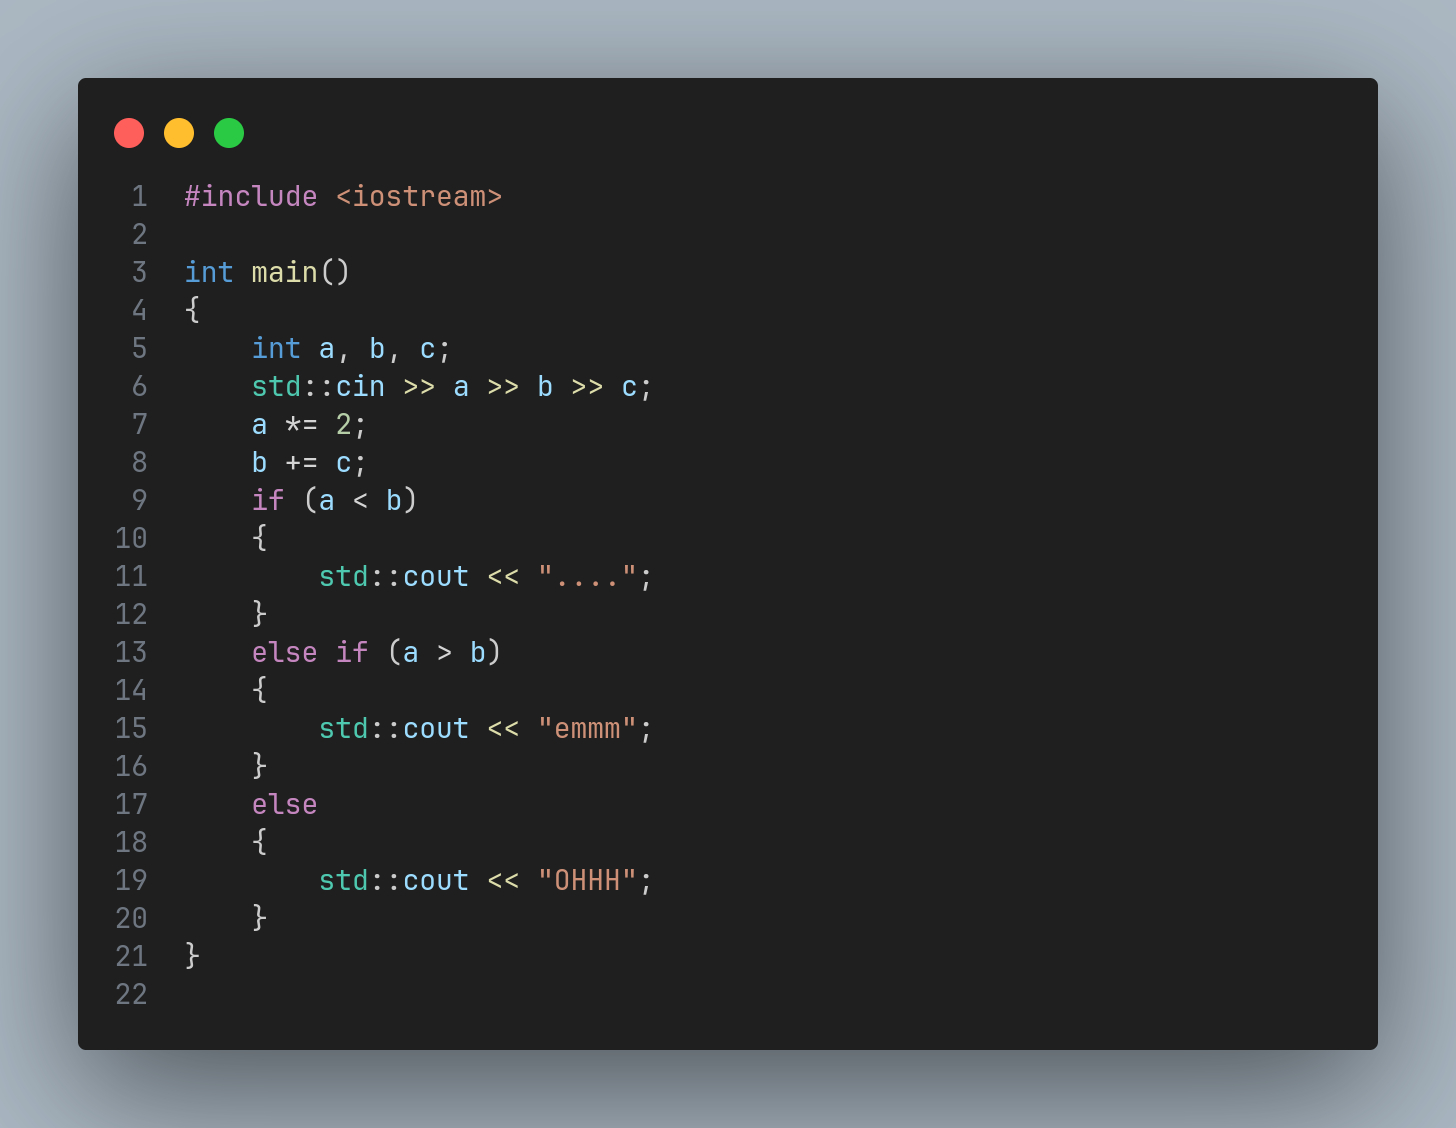
\includegraphics[scale=0.2]{images/std/A.png}
    \end{frame}

    \section{H}
    \hypertarget{H}{}
    \begin{frame}{\hyperlink{toc}{H.谷雨}\footnote{\href{https://acm816.cn/p/243}{\underline{补题链接}}}}
        \begin{block}{题目大意}
            \begin{itemize}
                \item 给定不同阶段的升级所需经验,求$0-K$的所需经验。
                \item 关键词:语法题(选择语句),签到
                \item 一血:70min
            \end{itemize}
        \end{block}
        \begin{itemize}
            \item 模拟即可。
            \item 对C/C++选手:请注意开long long。
        \end{itemize}
    \end{frame}
    \begin{frame}{std}
        \centering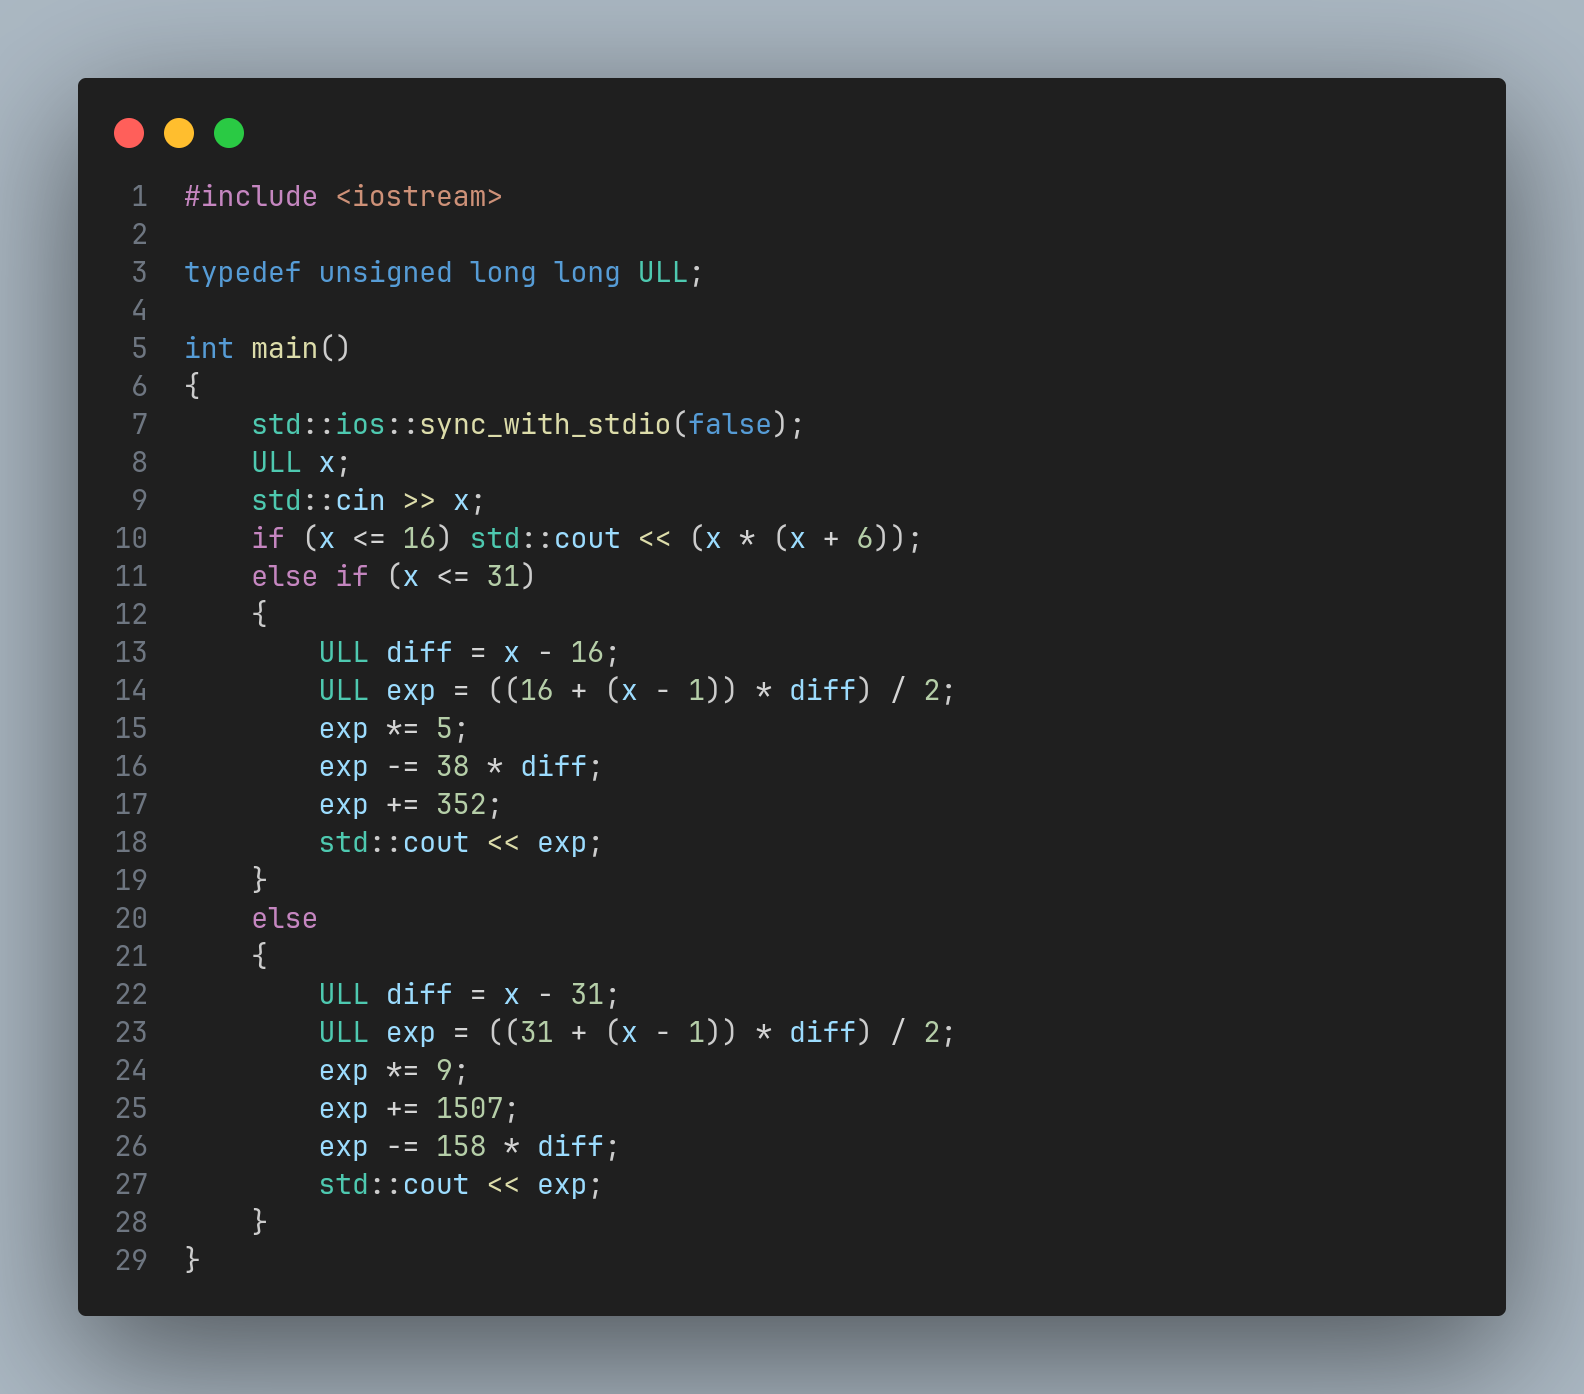
\includegraphics[scale=0.18]{images/std/H.png}
    \end{frame}

    \section{B}
    \hypertarget{B}{}
    \begin{frame}{\hyperlink{toc}{B.祝各位都能取得好成绩}\footnote{\href{https://acm816.cn/p/237}{\underline{补题链接}}}}
        \begin{block}{题目大意}
            \begin{itemize}
                \item 给定若干个单词,统计每个字母出现的次数。
                \item 关键词:语法题(数组),签到
                \item 一血:7min
            \end{itemize}
        \end{block}
        \begin{itemize}
            \item 将26个英文字母映射到数组下标并统计,输出数组即可。
        \end{itemize}
    \end{frame}
    \begin{frame}{std}
        \centering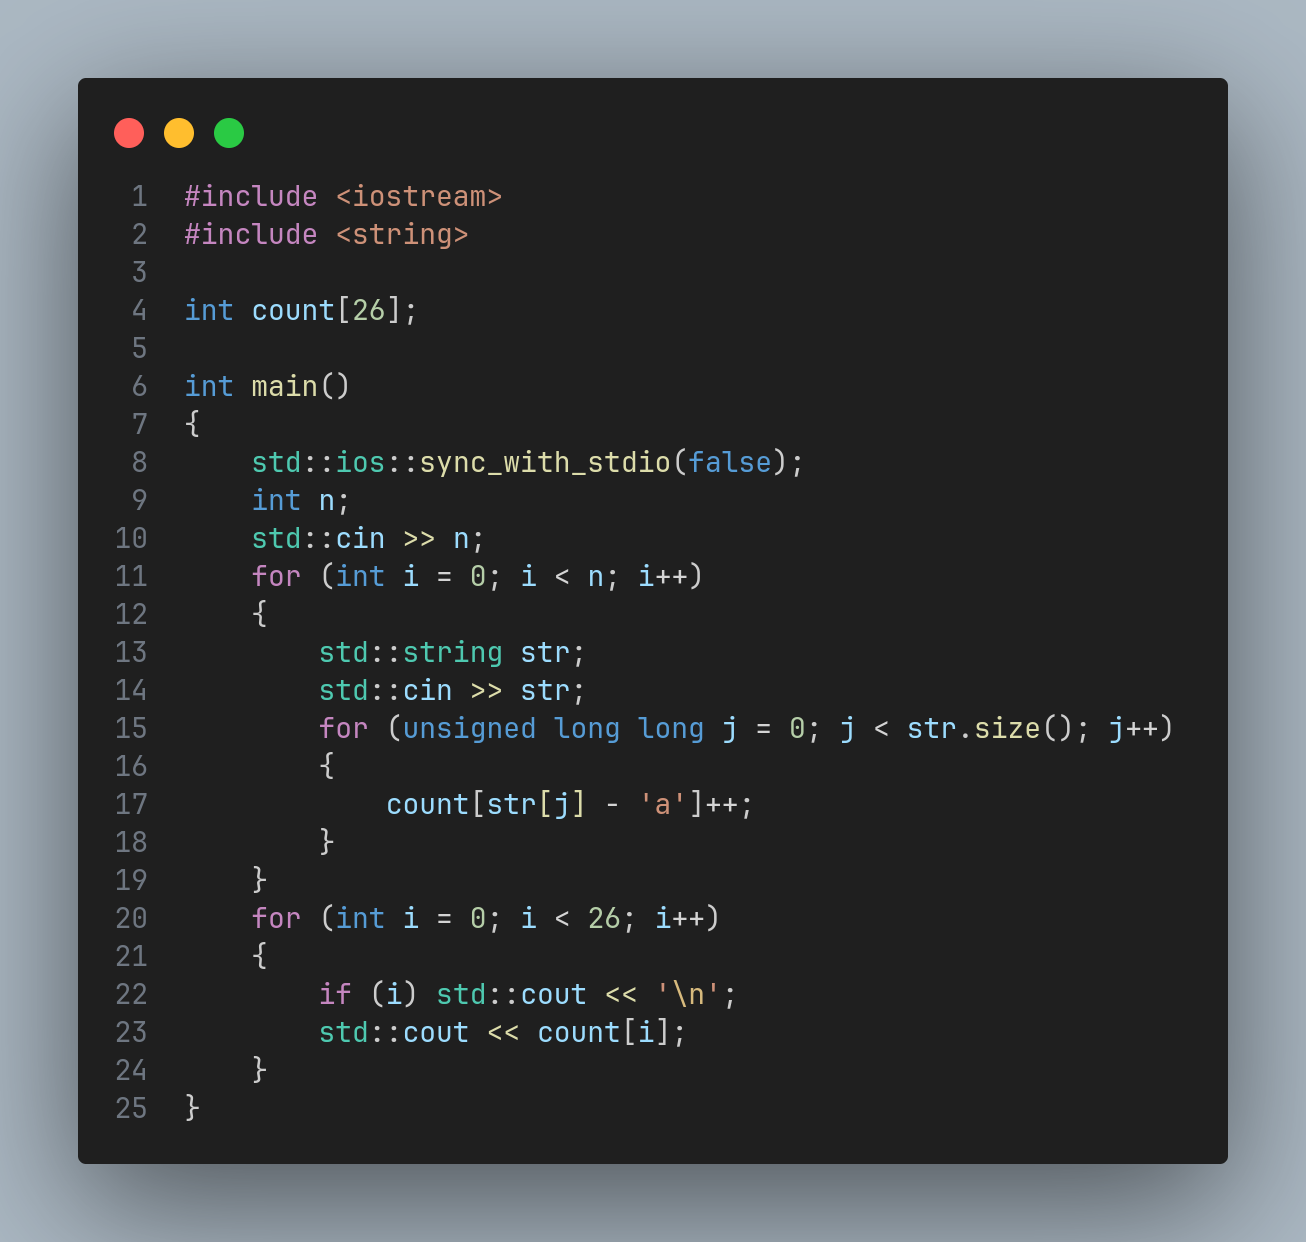
\includegraphics[scale=0.18]{images/std/B.png}
    \end{frame}

    \section{G}
    \hypertarget{G}{}
    \begin{frame}{\hyperlink{toc}{G.清明}\footnote{\href{https://acm816.cn/p/242}{\underline{补题链接}}}}
        \begin{block}{题目大意}
            \begin{itemize}
                \item 累加变量将顺序累加序列,要求任意时刻变量均大于$0$,求其初值。
                \item 关键词:前缀和,签到
                \item 一血:97min
            \end{itemize}
        \end{block}
        \begin{itemize}
            \item 顺序累加具有前缀性,因此使用前缀和计算每个状态。
            \item 若序列均为正数,答案为$1$。
            \item 若序列存在负数,则答案为前缀和中最小值的相反数$+1$。
            \item 对C/C++选手:请注意开long long。
        \end{itemize}
    \end{frame}
    \begin{frame}{std}
        \centering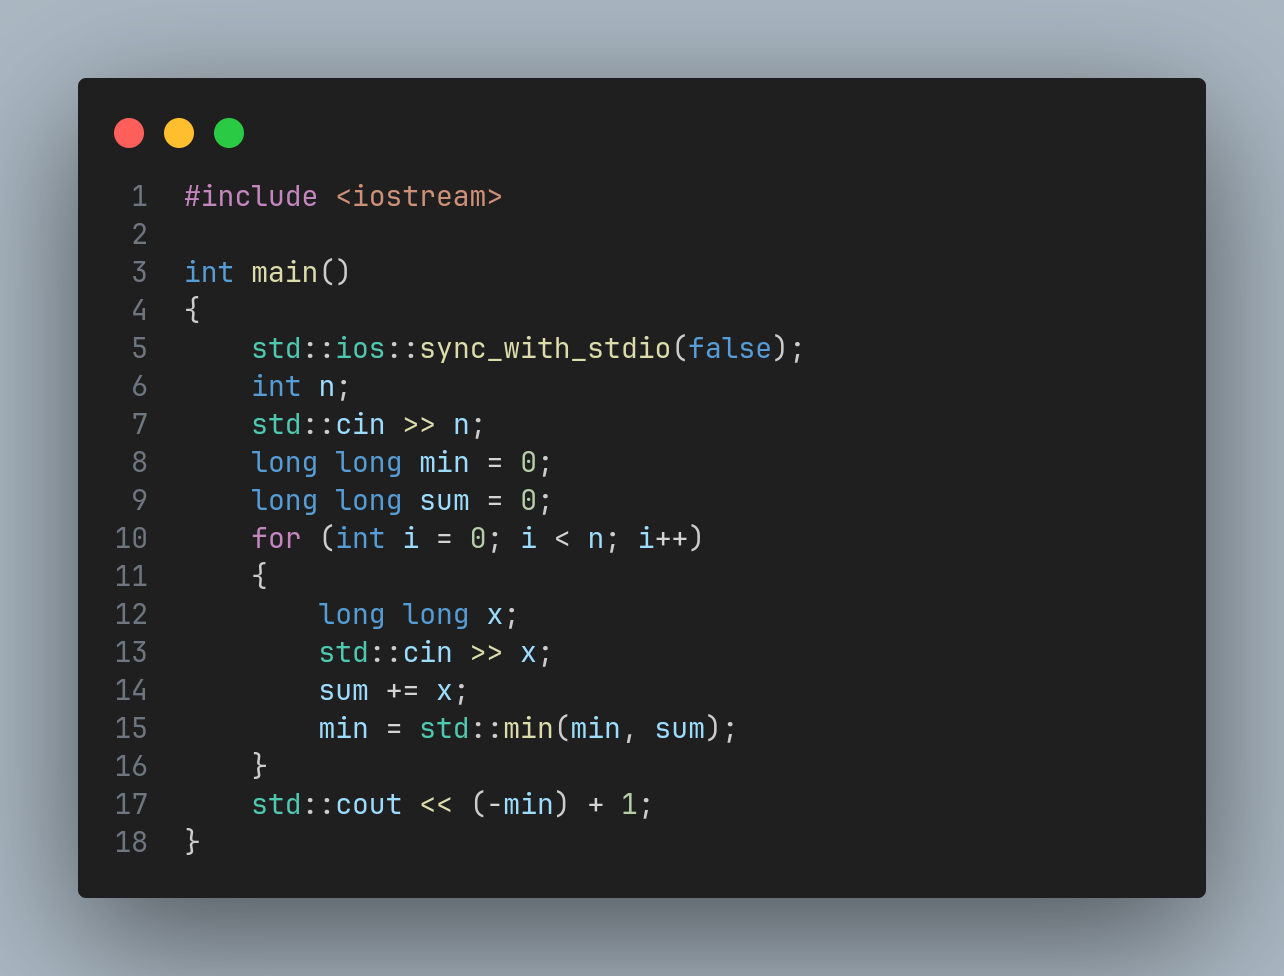
\includegraphics[scale=0.25]{images/std/G.png}
    \end{frame}
    \section{C}
    \hypertarget{C}{}
    \begin{frame}{\hyperlink{toc}{C.立春}\footnote{\href{https://acm816.cn/p/238}{\underline{补题链接}}}}
        \begin{block}{题目大意}
            \begin{itemize}
                \item 在二维网格上有若干个数字$14$,其将向上下左右方向上扩散,每扩散一次数字$-1$,当相遇时取较大值。输出扩散后的网格。
                \item 关键词:找规律/BFS
                \item 一血:53min
            \end{itemize}
        \end{block}
        本题为BFS模板题,不再赘述。下面介绍找规律方法:
        \begin{itemize}
            \item 
        \end{itemize}
    \end{frame}
\end{document}